% kuleuventheme2 by Janez Kren, September 2017, janez.kren@kuleuven.be, based on:
% kuleuventheme 1.3 by Roland Pastorino, 2013 roland.pastorino@kuleuven.be / www.rolandpastorino.com

\documentclass[11pt,t]{beamer}
\usetheme{kuleuven2}	%THEME OPTIONS for LOGO: kul (default), kulak, lrd,    ; OPTIONS for TITLE PAGE: normal (default), sedes


%%% OTHER SETTINGS
\usefonttheme[onlymath]{serif}			% math font with serifs, delete to make it sans-serif
\setbeamertemplate{footline}[body] 		% delete this line to remove footline bar on all frames
\usepackage[orientation=landscape,size=custom,width=16,height=9,scale=0.5,debug]{beamerposter} %enable for widescreen 16:9 ratio
%\titlegraphic{ \includegraphics[width=.2\paperwidth]{mytitlepagepic.png} } %optional title page image


%%% ADDED PACKAGES:
\usepackage[english]{babel}
\usepackage{amsfonts}
\usepackage{amssymb}


%%% TITLE PAGE INFO:
\title[Distributed Adversarial Attacks]{Distributed Adversarial Attacks} %[]] will appear in footline
\subtitle{Intermediate presentation}

\author{Sander Prenen}
\institute{KU Leuven}
\date{December 2021}




\begin{document}
\csname beamer@calculateheadfoot\endcsname %recalculate head and foot dimension

% Title page
\begin{frame}[plain,noframenumbering]
	\titlepage
\end{frame}

% Table of Contents
\begin{frame}{Outline}
	\hfill	{\large \parbox{.961\textwidth}{\tableofcontents[hideothersubsections]}}
\end{frame}

\section{Research topic}
\begin{frame}{Research topic}
\begin{itemize}
	\item Black-box adversarial attack
	\begin{itemize}
		\item Decision based
		\item No confidence scores
	\end{itemize}

	\item Distribution
	\begin{itemize}
		\item Particle swarm optimization (PSO)
	\end{itemize}
\end{itemize}
\end{frame}

\subsection{Related work}
\begin{frame}{Related work}
\begin{itemize}
	\item Boundary attack (BA)
	\vspace{6pt}
	\begin{figure}
	\centering
	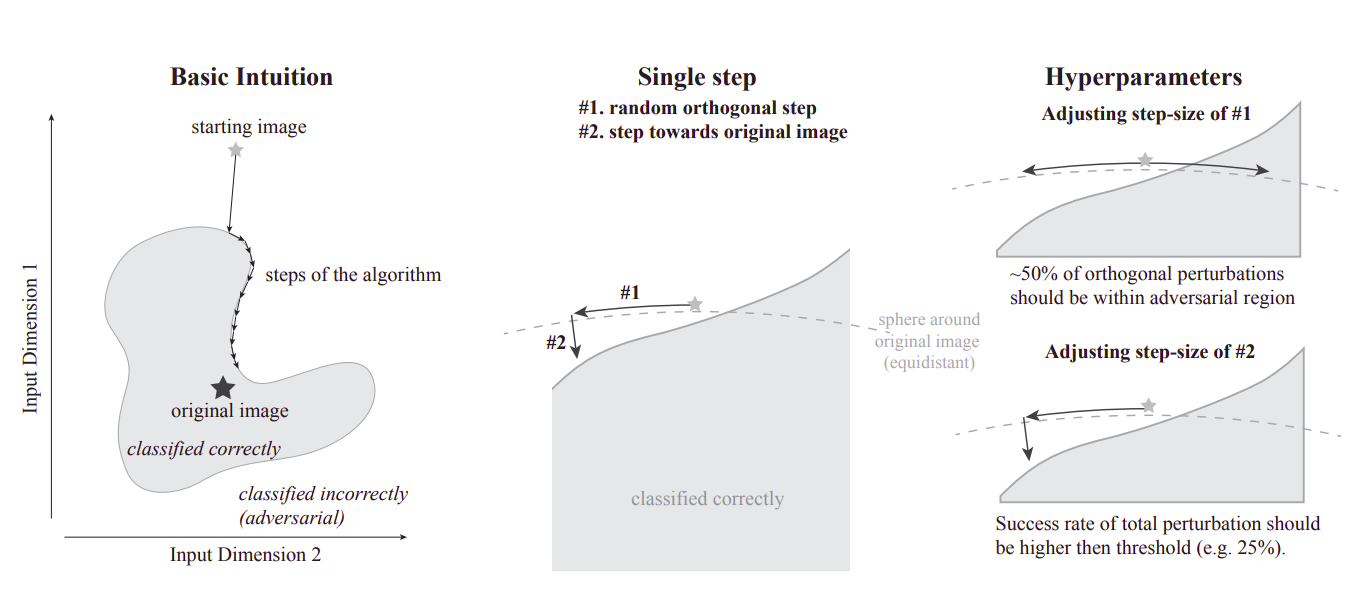
\includegraphics[width=0.8\textwidth]{graphics/boundary_attack.png}
	\caption{Boundary attack \cite{brendel2018decisionbased}\label{fig:boundary_attack}}
	\footnotesize
	\flushleft
	\end{figure}
\end{itemize}

\end{frame}

\begin{frame}{Related work}
\begin{itemize}
	\item Boundary attack (BA)
	\item Biased boundary Attack (BBA)
	\begin{itemize}
		\item Masking
		\item Perlin noise
	\end{itemize}
\end{itemize}
\end{frame}

\begin{frame}{Related work}
\begin{itemize}
	\item HopSkipJump attack (HSJA)
	\vspace{6pt}
	\begin{figure}
	\centering
	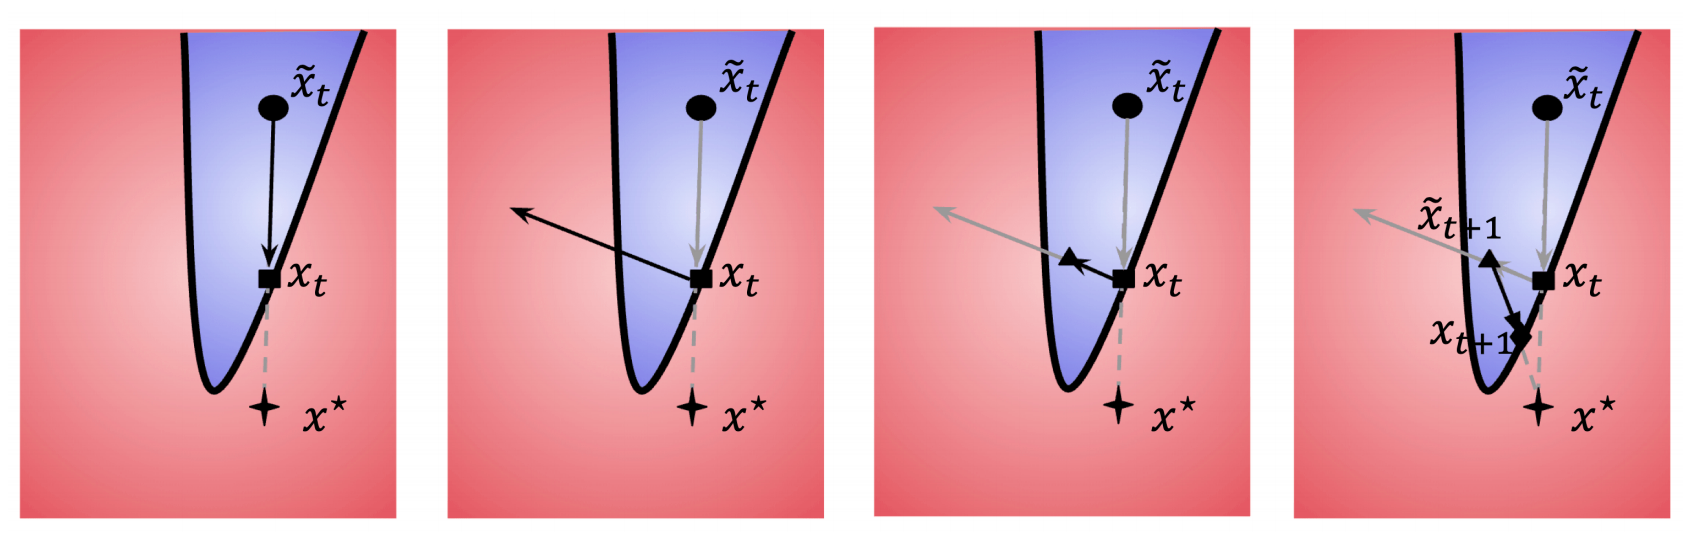
\includegraphics[width=0.8\textwidth]{graphics/hsj_attack.png}
	\caption{HopSkipJump attack \cite{chen2020hopskipjumpattack}\label{fig:hsj_attack}}
	\footnotesize
	\flushleft
	\end{figure}
\end{itemize}
\end{frame}

\subsection{Research gap}
\begin{frame}{Research gap}
\begin{itemize}
	\item Stateful detection
	\begin{figure}
	\centering
	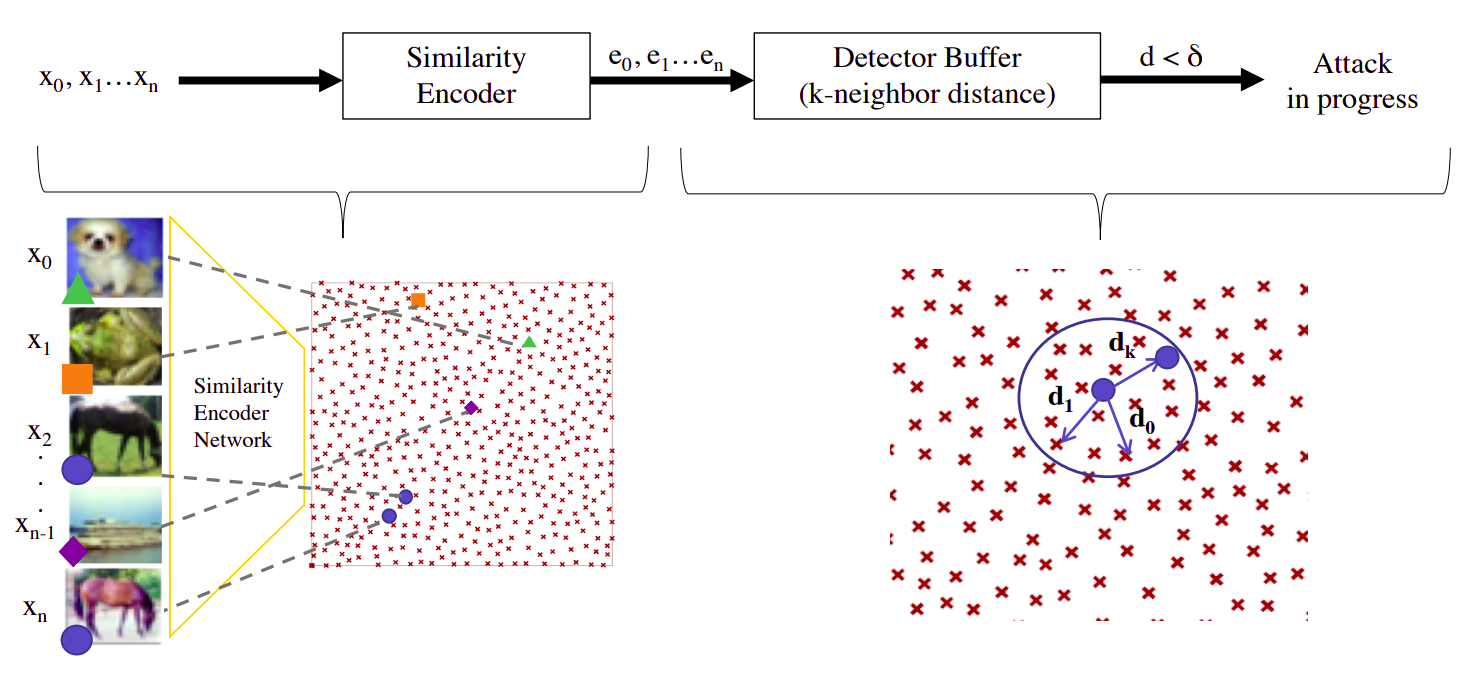
\includegraphics[width=0.8\textwidth]{graphics/stateful_detection.png}
	\caption{Stateful detection \cite{chen2019stateful}\label{fig:stateful_detection}}
	\footnotesize
	\flushleft
	\end{figure}
\end{itemize}
\end{frame}

\begin{frame}{Research gap}
\begin{itemize}
	\item Stateful detection
	\begin{itemize}
		\item Assumption: attack done by \alert{one} user/account/IP
		\item No cooperation between users
	\end{itemize}
	
	\item Distribution
	\begin{itemize}
		\item Evade the stateful detection algorithm
		\item Cooperate to craft better adversarial examples in fewer queries
	\end{itemize}
	
	\item Existing work
	\begin{itemize}
		\item Uses confidence scores \cite{10.1007/978-3-030-59013-0_22, s20247158}
	\end{itemize}
\end{itemize}
\end{frame}

\subsection{Research questions}
\begin{frame}{Possible research questions}
	\begin{exampleblock}
	{Can PSO be used to craft adversarial examples in a decision based setting?}
	\end{exampleblock}
	\begin{exampleblock}
	{Can PSO be used to craft the global best adversarial example in a decision based setting?}
	\end{exampleblock}
	\begin{exampleblock}
	{Can distribution of queries help towards evading stateful detection mechanisms?}
	\end{exampleblock}
	\begin{exampleblock}
	{What distribution scheme triggers the least detections by a stateful detection mechanism?}
	\end{exampleblock}

\end{frame}

\section{Progress}
\begin{frame}{Progress}
\begin{itemize}
	\item Working PSO algorithm based on Biased boundary attack (PSO-BA)
	\begin{figure}
	\centering
	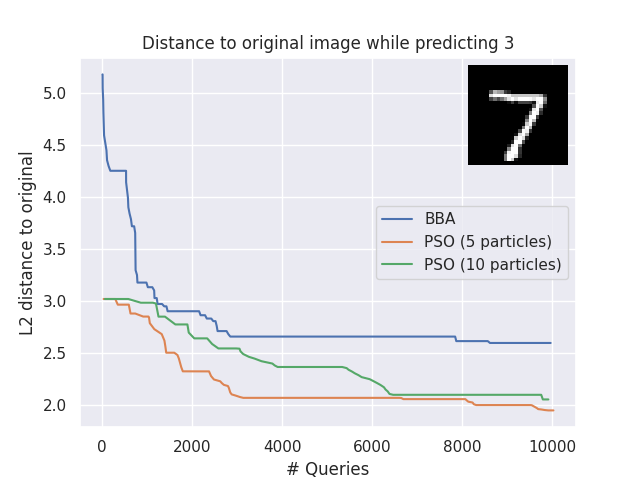
\includegraphics[width=0.30\textwidth]{graphics/comparison_1_3.png}
	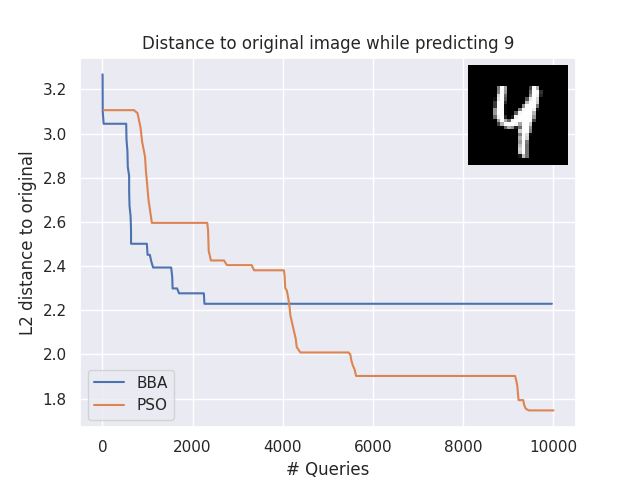
\includegraphics[width=0.30\textwidth]{graphics/comparison_42_9.png}
	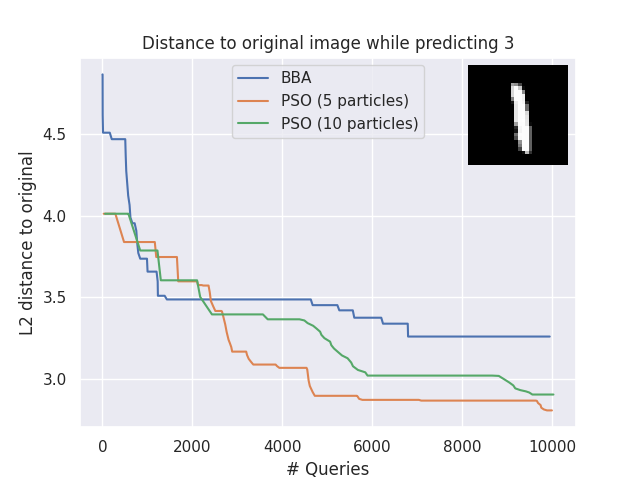
\includegraphics[width=0.30\textwidth]{graphics/comparison_1302_3.png}
	\caption{Comparison BBA and PSO-BA\label{fig:comparisons}}
	\footnotesize
	\flushleft
	\end{figure}
\end{itemize}
\end{frame}

\begin{frame}[plain]{Progress}
\begin{itemize}
	\item Working PSO algorithm based on Biased boundary attack (PSO-BA)
	\item Performed experiments to show that PSO is a viable candidate
	\begin{figure}
	\centering
	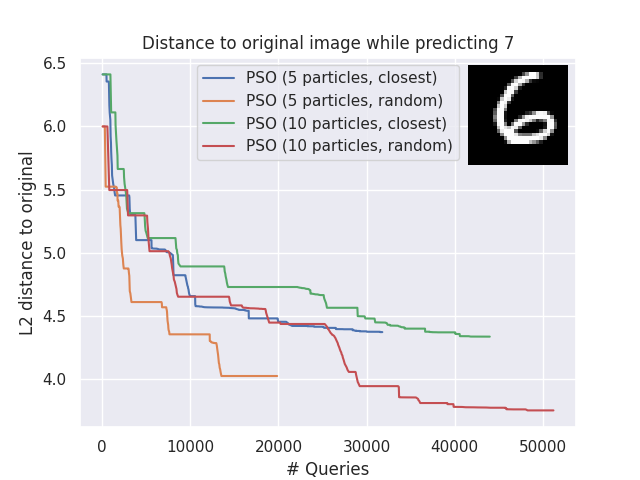
\includegraphics[width=0.45\textwidth]{graphics/random_vs_closest.png}
	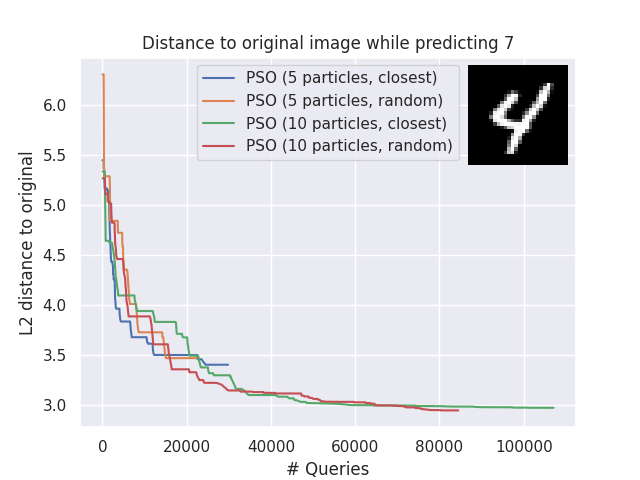
\includegraphics[width=0.45\textwidth]{graphics/random_vs_closest_1.png}
	\caption{Comparison random versus closest initialization\label{fig:rand_vs_close}}
	\footnotesize
	\flushleft
	\end{figure}
\end{itemize}
\end{frame}

\begin{frame}{Progress}
\begin{itemize}
	\item Working PSO algorithm based on Biased boundary attack (PSO-BA)
	\item Performed experiments to show that PSO is a viable candidate
	\item Compare detections PSO-BA and BBA (Not done yet but hopefully have done this before the presentation)
\end{itemize}
\end{frame}

\section{Future work}
\begin{frame}{Future work}
\begin{itemize}
	\item Improving the existing PSO-BA
	\begin{itemize}
		\item Implementing different distribution schemes and comparing the number of detections
		\item Tuning the hyperparameters to minimize detections
		\item Performing more experiments to confirm the results
		\item Applying the algorithm on different datasets
	\end{itemize}
	\item Implementing a new algorithm based on PSO and HSJA
	\begin{itemize}
		\item Comparing this algorithm with PSO-BA
	\end{itemize}
\end{itemize}
\end{frame}

\begin{frame}[c,plain,noframenumbering]
\begin{tikzpicture}[remember picture,overlay]
\fill[fill=kul-blue]
    (current page.south east)  rectangle  ([shift={(0,-0.1\paperheight)}]current page.north west)   ;
\end{tikzpicture}

\centering
\textcolor{white}{Questions?}
\end{frame}

\appendix
\section*{References}
\begin{frame}[allowframebreaks]{References}
\bibliographystyle{unsrt}
\bibliography{citations.bib}
\end{frame}
\end{document}